To evaluate our algorithm's performance a number of experiments were run on both the Euler and the
Piz Daint cluster. In the following paragraphs we will first describe both the Euler and the Piz
Daint setups. We will then go on to discussing each experiment separately. The errorbars in all plots refer to a 95\% confidence interval.

\mypar{Euler setup}
Each node in the Euler V cluster contains two 12-core Intel Xeon Gold 5118 processors and 96 GB of
DDR4 memory clocked at 2400 MHz \cite{Euler}. We were allowed to use up to two nodes, giving us a
maximum of 48 cores. The algorithm was compiled and run using gcc 6.2.3 and Open MPI 3.0.0.

\mypar{Piz Daint setup}
Each of the utilized XC40 nodes on Piz Daint contains two Intel Xeon E5-2695, each with 18 hardware
threads,
and 32 GB of DDR4 memory. We used both gcc and the Cray compiler, and observed marginally faster
run times with the latter.

\mypar{Graph Generation}
Our algorithm was evaluated on undirected, unweighted graphs. Multiple edges connecting the same
two vertices and self loops were not allowed. All graphs were generated using \cite{Parmat}. The same tool was used in \cite{comm_avoiding}

\mypar{MPI vs OMP vs Communication Avoiding}

\newlength{\fsize}
\setlength{\fsize}{0.45\textwidth}
\begin{figure}%[H]

\begin{subfigure}[c]{\fsize}
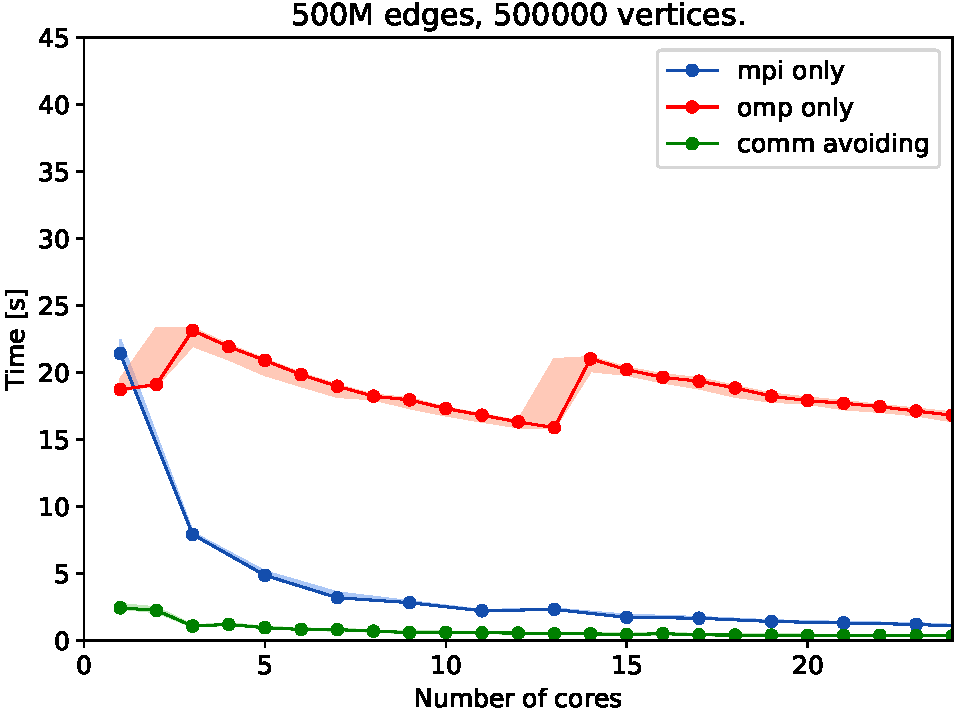
\includegraphics[width=\textwidth]{data/50000our_impl}
\subcaption{$5\times10^{5}$ vertices}
\label{fig:mpi_omp_commavoiding_euler_1}
\end{subfigure}

\begin{subfigure}[c]{\fsize}
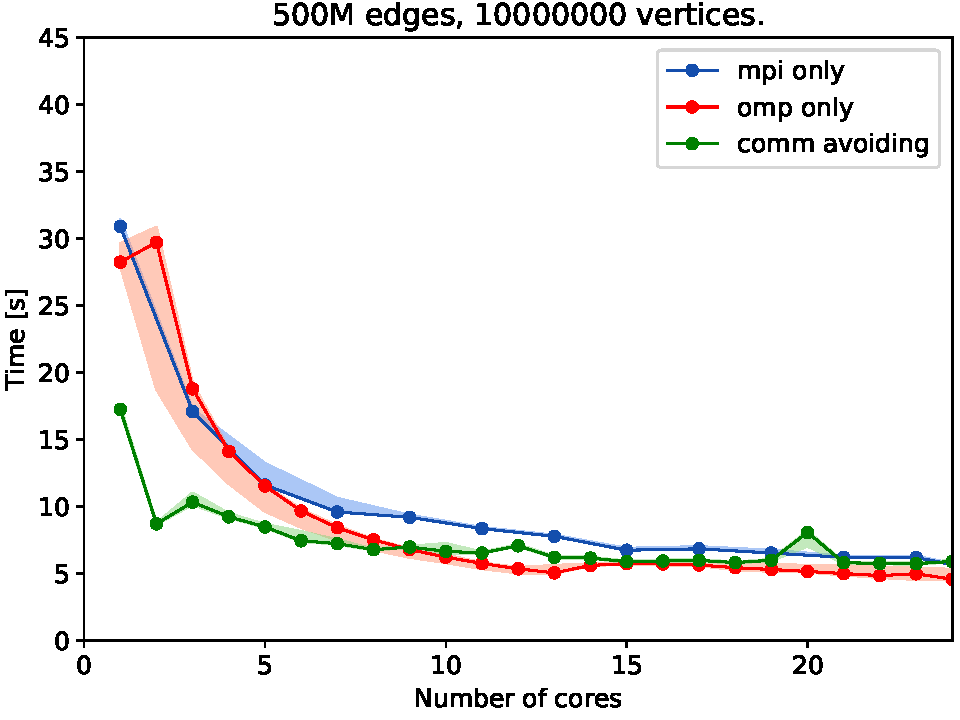
\includegraphics[width=\textwidth]{data/10000our_impl}
\subcaption{$10^{7}$ vertices}
\label{fig:mpi_omp_commavoiding_euler_2}
\end{subfigure}

\begin{subfigure}[c]{\fsize}
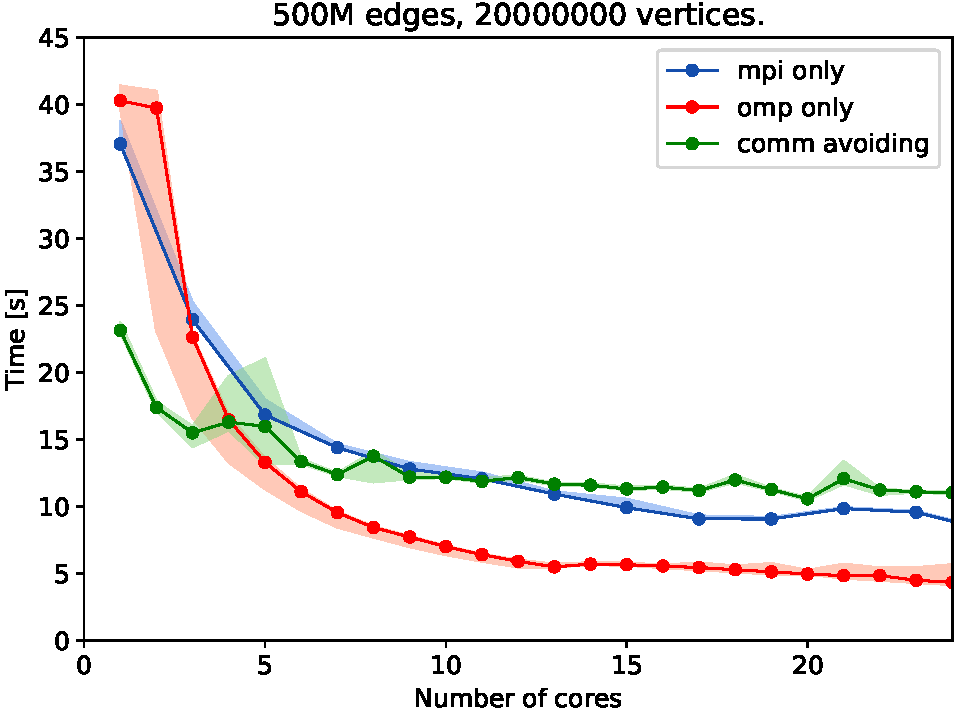
\includegraphics[width=\textwidth]{data/20000our_impl}
\subcaption{$2\times10^{7}$ vertices}
\label{fig:mpi_omp_commavoiding_euler_3}
\end{subfigure}

\caption{Comparison of the total runtime of our algorithm with the communication avoiding algorithm
\cite{comm_avoiding} over three different graphs each with $5\times10^{8}$ edges and $5\times10^5,
1\times10^7, 2\times10^7$ vertices. The experiment was run on the Euler
cluster.}
\label{fig:mpi_omp_commavoiding_euler}
\end{figure}

The results in \autoref{fig:mpi_omp_commavoiding_euler} show our algorithm compared with the
communication avoiding algorithm \cite{comm_avoiding} on three different graphs with the same
number of edges but different densities. Our algorithm was run in MPI and OMP only mode.\\
\autoref{fig:mpi_omp_commavoiding_euler_1} shows the MPI version outperforming the OMP version
on the densest graph. This can be explained by the combination of two effects. The first is that a
dense graph results in more contention between the OMP threads during the
edge contractions. The second is that the reduction scales linearly with the number of vertices.
Since the number of vertices is comparatively low in a dense graph the
reduction is fast. For the OMP version we further observe a significant increase in total
compute time from one to two cores and from 12 to 13 cores. The first jump can be explained by the
initial overhead of doing the computation in parallel. Since a single CPU on Euler has 12 cores the
second jump is a result of  the cache coherency protocol being slow across multiple CPUs.\\
The results in \autoref{fig:mpi_omp_commavoiding_euler_2} and
\autoref{fig:mpi_omp_commavoiding_euler_3} were obtained using sparser graphs compared to
\autoref{fig:mpi_omp_commavoiding_euler_1}. Here, for a large number of cores, the OMP version
is clearly faster than the MPI version. \autoref{fig:mpi_omp_commavoiding_euler} shows a trend
of the OMP version speeding up as the graph becomes sparser, while the MPI version slows
down. The OMP version's speed up can be explained by less contention between the OMP
threads due to the sparser graph. The MPI version's slow down is the result of the increased
reduction time due to the larger number of vertices.\\
The results in \autoref{fig:mpi_omp_commavoiding_euler} show the communication avoiding algorithm
scaling badly with the number of cores. This is expected since the edge contractions are computed
on a single node. Since our algorithm does scale with the number of cores up
to some point we manage to outperform the communication avoiding algorithm on each graph.

%
%\mypar{Mixing MPI and OMP}
%
%\begin{figure}%[H]
%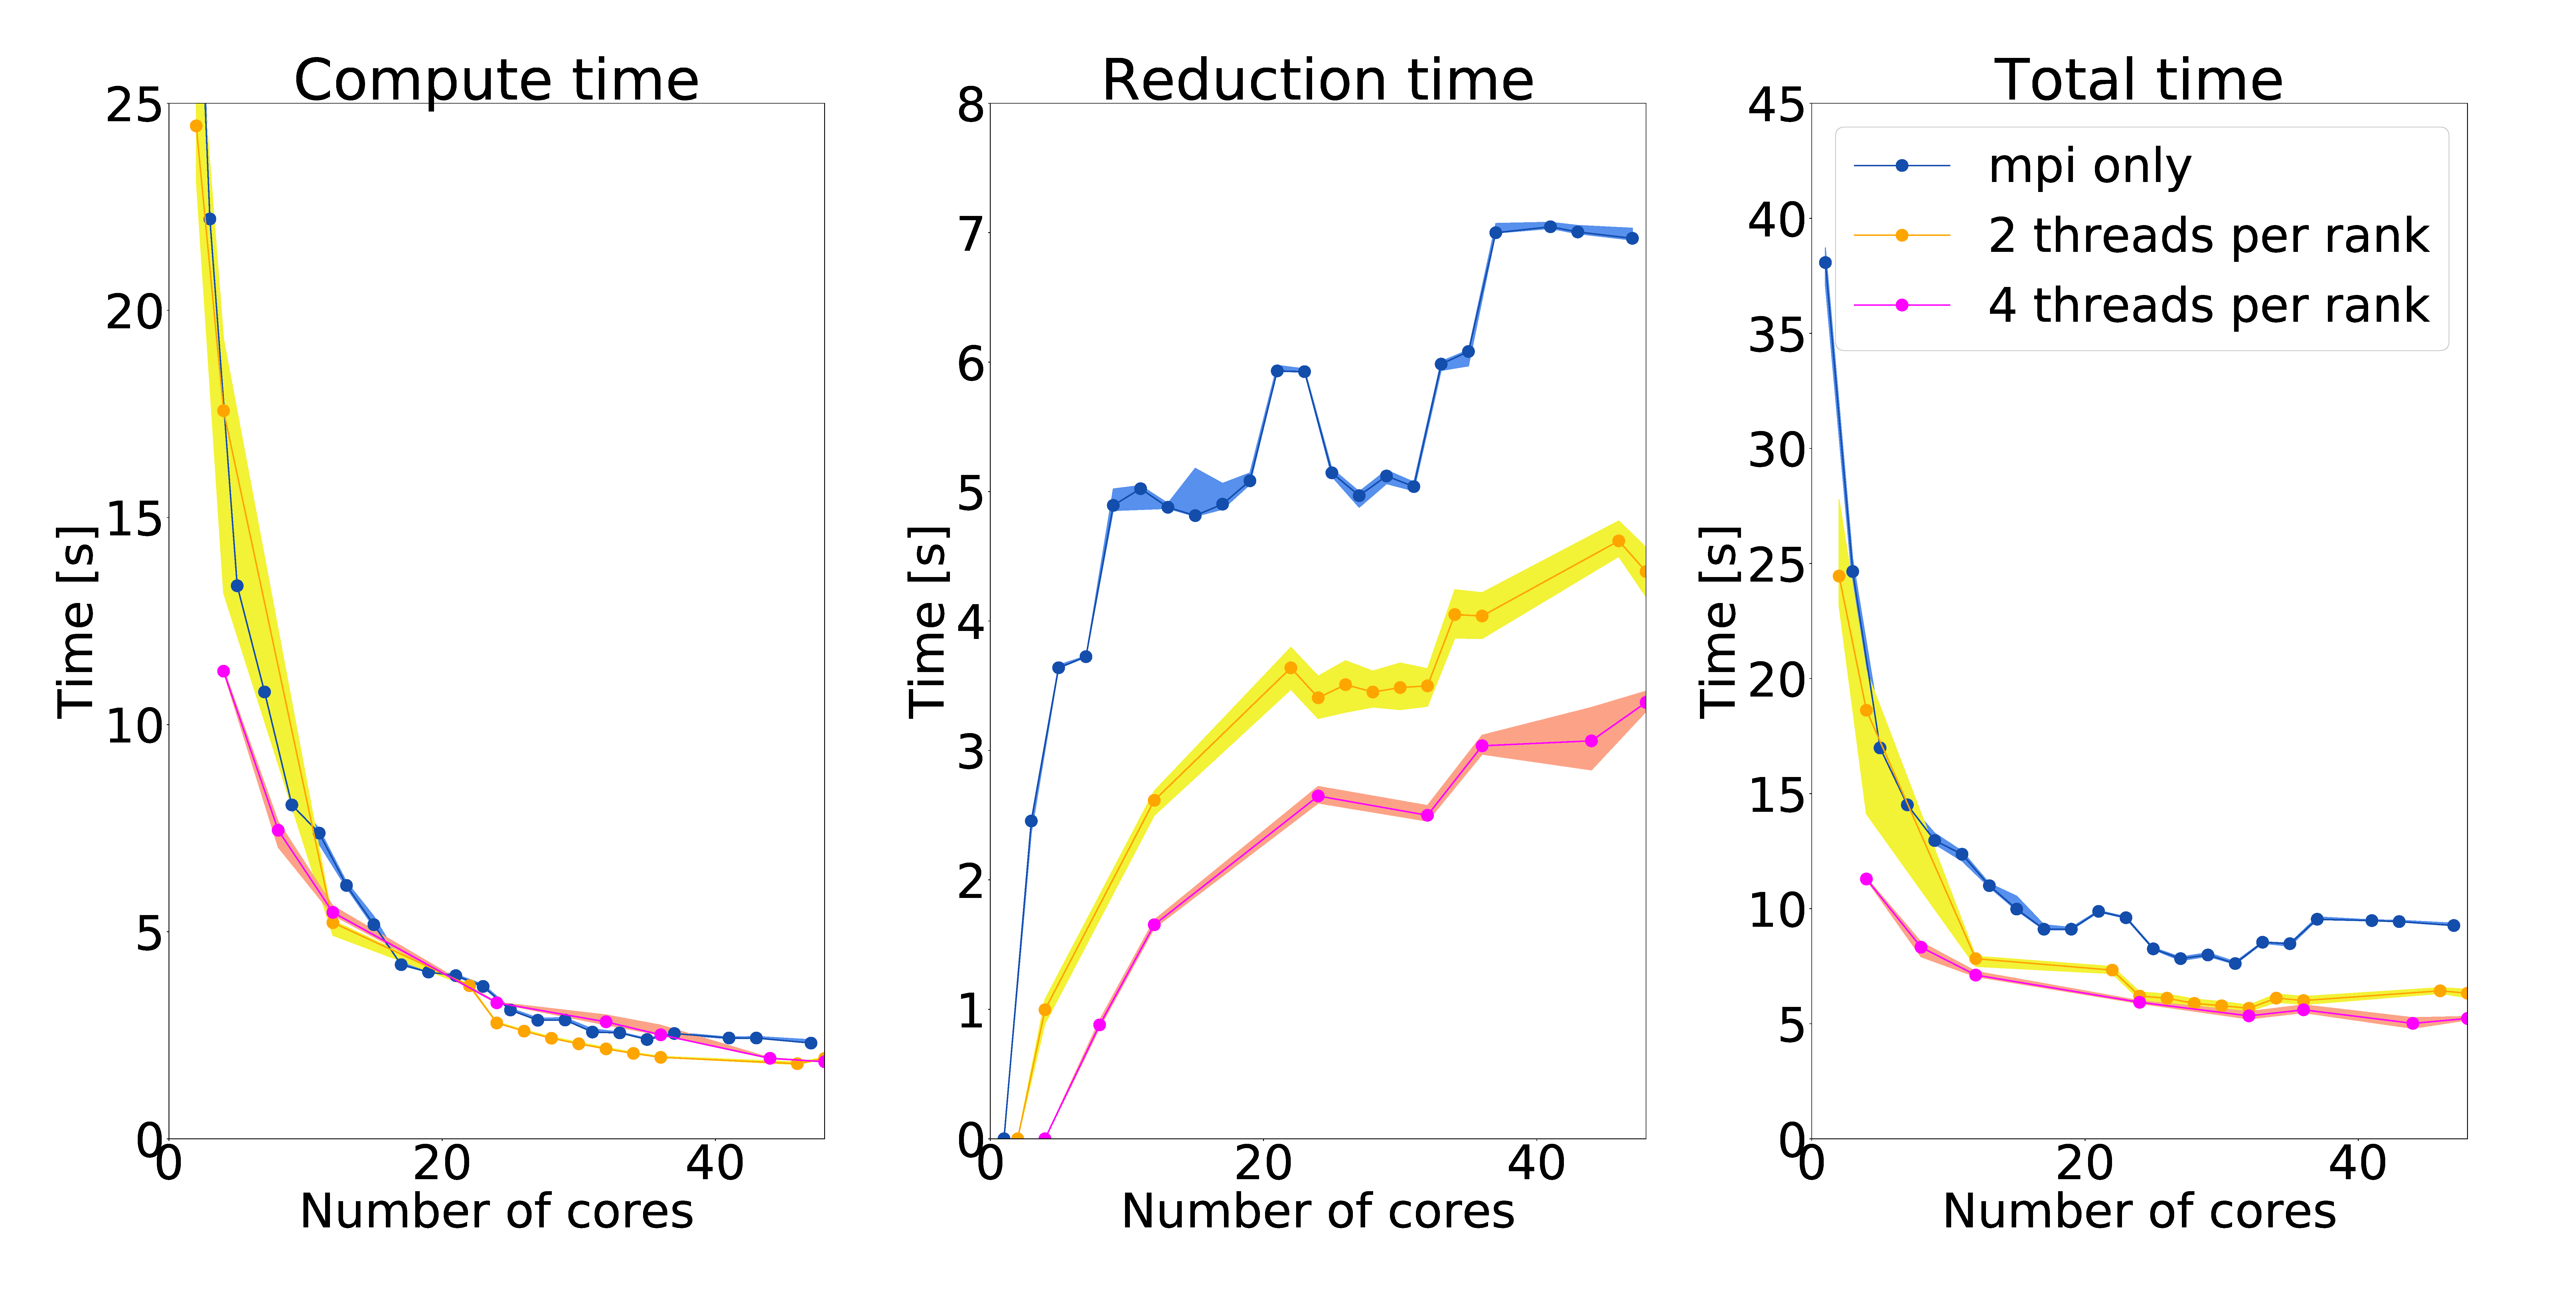
\includegraphics[width=0.5\textwidth]{plots/20000mpi_mixtures_with_everything}
%\subcaption{$2\times10^{7}$ vertices}
%\caption{Total runtime breakdown on graph with $5\times10^{8}$ edges and $2\times10^{7}$ vertices.
%The experiment was run on the Euler cluster.}
%\label{fig:mixed_euler}
%\end{figure}
%
%To further investigate the distinct difference between the MPI only and the OMP only version the
%algorithm was tested using a mixture of MPI and OMP.
%\autoref{fig:mixed_euler} shows the compute time being largely independent of the mixture. This is
%a consequence of the graphs sparsity which results in low contention between the OMP threads. The
%reduction time, however, wildly differs for the different mixtures. For each mixture it increases
%logarithmically with the number of MPI ranks. This results in the algorithm's performance
%decreasing as less OMP threads per MPI rank are used.


\mypar{Results on Piz Daint}

\begin{figure}%[H]
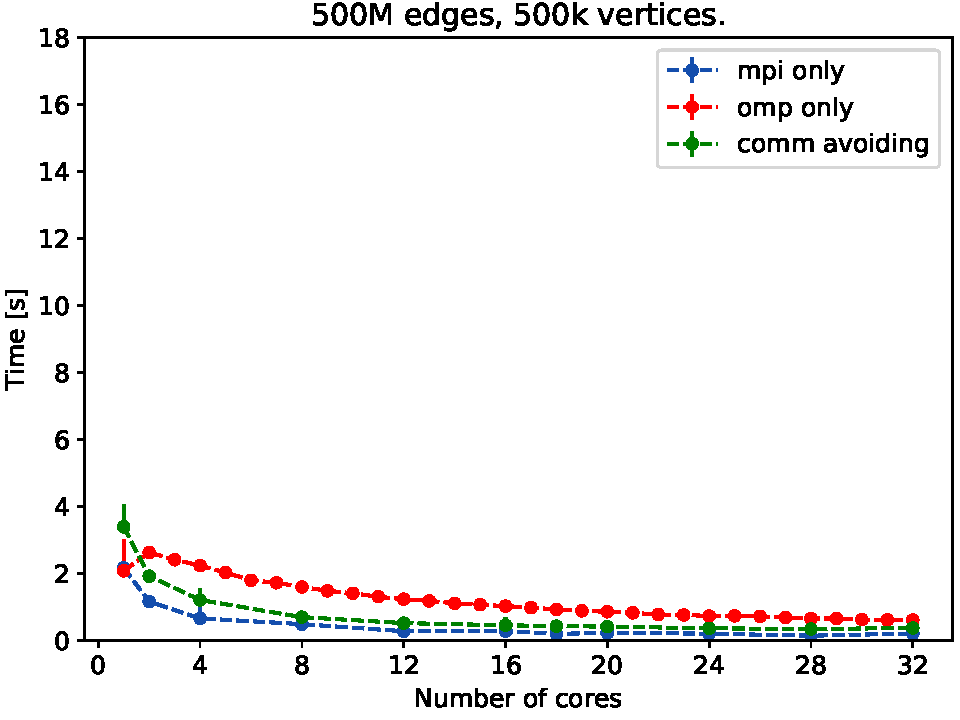
\includegraphics[width=\fsize]{data/plot_vertices_500k.pdf}
\caption{Piz Daint results on graph with $5\times10^8$ edges and $5\times10^5$ vertices.}
\label{fig:mpi_omp_commavoiding_daint_1}
\end{figure}

\begin{figure}%[H]
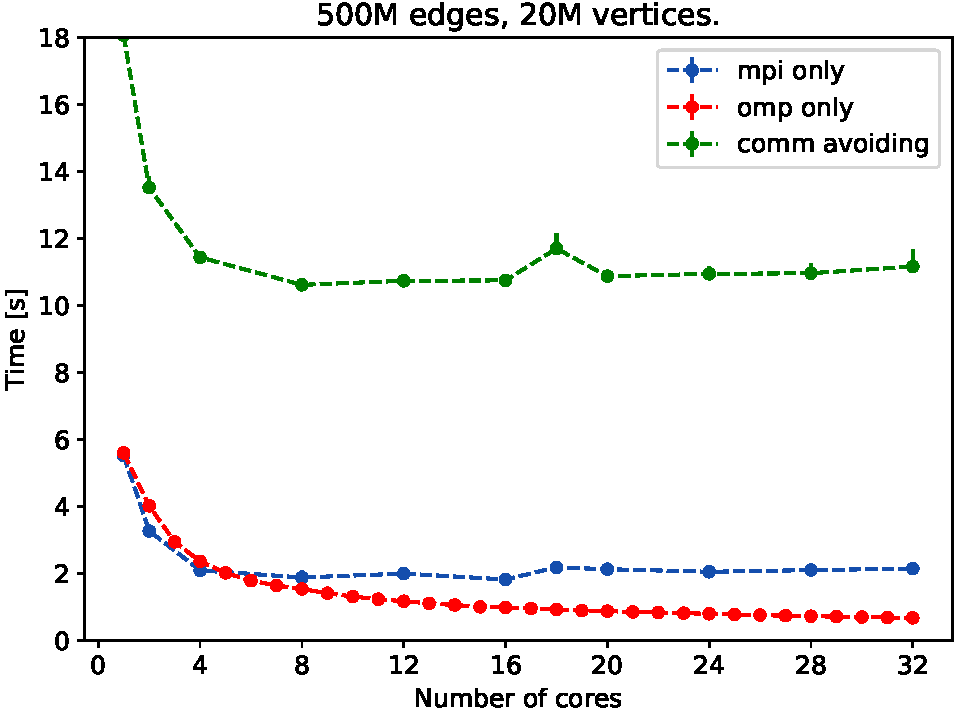
\includegraphics[width=\fsize]{data/plot_vertices_20M.pdf}
\caption{Piz Daint results on graph with $5\times10^8$ edges and $2\times10^7$ vertices.}
\label{fig:mixed_daint}
\end{figure}

Additionally we tested our algorithm on the Piz Daint cluster. The graphs used were the same as in
the experiments run on Euler. We will now discuss interesting differences in the results.\\
\autoref{fig:mpi_omp_commavoiding_daint_1} shows the results for the densest graph on Piz Daint.
The OMP version behaves differently compared to Euler. We still observe a decrease in performance
when going from one to two cores. The decrease is not as severe as on Euler. The performance
decrease as we go from one to multiple CPUs is no longer present. This can be explained by Daint's
cache coherency protocol being more efficient, especially across multiple CPUs.
\autoref{fig:mixed_daint} shows the Piz Daint results for different mixtures of MPI and OMP on the
sparsest graph. As on Euler, we do see the OMP version performing best for a large number of cores.
For all versions, except the OMP version, we can clearly see the effect the number of reduction
steps has on the runtime. It is most noticeable as we go from 16 to 18 cores. Here each version has
to perform an additional reduction step which results in the increased runtime.





\mypar{Speedups}

\begin{figure}%[H]
\begin{subfigure}[c]{\fsize}
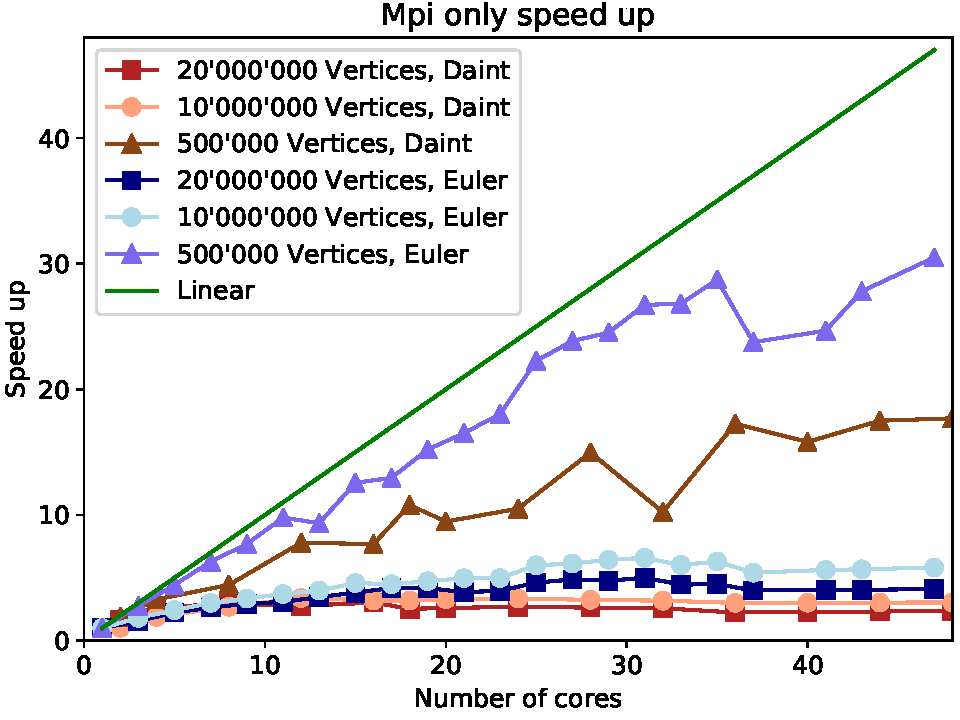
\includegraphics[width=\textwidth]{data/mpi_speedup_with_ref}
\subcaption{MPI only}
\label{fig:speedup_mpi}
\end{subfigure}
\begin{subfigure}[c]{\fsize}
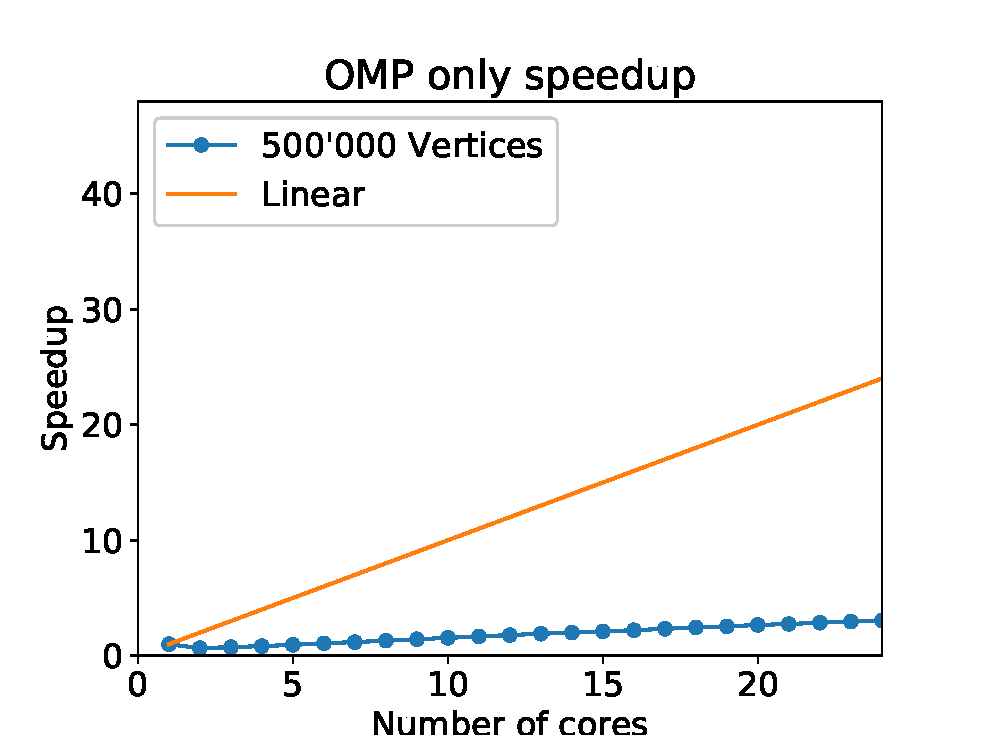
\includegraphics[width=\textwidth]{data/omp_speedup_with_ref}
\subcaption{OMP only}
\label{fig:speedup_omp}
\end{subfigure}
\caption{Speedup of MPI only and OMP only version on three different graphs each with
$5\times10^{8}$ edges.}
\label{fig:speedup}
\end{figure}

\autoref{fig:speedup} shows the measured speed up of the MPI and OMP version. As one
would expect from the results discussed previously the MPI version achieves better scaling on dense
graphs while the OMP version scales better on sparse graphs.\\
We can also see that our algorithm achieves better scaling on Euler for the MPI version. The reason
our algorithm scales better on Euler is that the single core performance is lower on Euler compared
to Daint. This means that the edge contractions dominate the runtime for longer before the
reduction step starts to be an issue.\\
For the OMP version the discrepancy in the speed ups can be explained by the differences in the
shared memory architecture.

\mypar{Distributed vertices}
As the performance of the RMA controller is essential, we tested the distributed vertices algorithm only on Piz Daint.
In \autoref{fig:distributed_scaling} we report the weak scaling for an input with 400M vertices per
process, 18 threads per process, and 200M edges.

While the scaling for this specific case is excellent, this works only when the average connected component size is
extremely small. Due to development time constraints each MPI operation is
synchronized locally, hurting the performance in cases where several RMA operations are required to obtain the
root of a tree.

\begin{figure}%[H]
    \includegraphics[width=\fsize]{plots/weak_scaling.pdf}
    \caption{Weak scaling on Piz Daint of the distributed vertices algorithm. Each process is run
    on a single socket.}
    \label{fig:distributed_scaling}
\end{figure}
